\section{Webanwendung zur Veranstaltungsorganisation}

Die entwickelte Webanwendung unterstützt Veranstalter und Schausteller bei der Organisation von Events. Veranstalter können eigenständig Events erstellen, Bewerbungen verwalten und Verträge abschließen. Schausteller haben die Möglichkeit, sich über die Plattform für Events zu bewerben und ihre Teilnahme zu organisieren.

\subsection{Motivation für die Wahl der Webanwendung als Fallstudie}

Diese Webanwendung wurde als Fallstudie gewählt, weil sie mehrere zentrale Herausforderungen der Softwareentwicklung abbildet. Die Plattform erfasst komplexe organisatorische Abläufe. Sie unterstützt Veranstalter bei der Verwaltung von Events und Schausteller bei der Bewerbung und Vertragsabwicklung. Beide Nutzergruppen haben unterschiedliche, aber miteinander verknüpfte Interaktionen mit dem System. Die Anwendung bietet vielfältige Testfälle, um verschiedene Teststrategien systematisch zu vergleichen. Durch ihre praxisnahe Umsetzung dient sie als reales Beispiel für die digitale Transformation im Veranstaltungsmanagement.

Ein persönlicher Grund für die Entwicklung dieser Webanwendung war eine reale Erfahrung. Ein Bekannter berichtete, dass er jedes Jahr seinen Foodtruck für eine Veranstaltung anmelden musste. Der Bewerbungsprozess verlief ausschließlich analog. Er musste den Veranstalter kontaktieren, viele E-Mails schreiben und zahlreiche Telefonate führen. Die vertraglichen Details wurden ebenfalls manuell geklärt. Dieser Prozess war aufwendig und fehleranfällig. Es war schwierig, den Überblick über alle Bewerbungen und abgeschlossenen Verträge zu behalten. Daraus entstand die Idee, eine digitale Lösung zu entwickeln. Eine Plattform sollte alle Bewerbungen und Verträge zentral speichern. Der Bewerbungsprozess sollte mit wenigen Klicks erfolgen. Verträge sollten direkt digital erstellt und verwaltet werden. Veranstalter sollten neue Events effizient organisieren können. Viele Veranstaltungen sind weiterhin analog und verfügen über keine zentrale digitale Lösung. Diese Webanwendung bietet eine einheitliche Plattform für Veranstalter und Schausteller.

\subsection{Bewerbungsprozess}

Schausteller können sich über vorhandene Events informieren und sich direkt über die Plattform bewerben. Veranstalter können die eingegangenen Bewerbungen einsehen und den aktuellen Status jeder Bewerbung nachverfolgen. Das System zeigt an, ob eine Bewerbung neu eingereicht, akzeptiert oder bereits in einen Vertrag überführt wurde. Wird eine Bewerbung angenommen, kann der Veranstalter daraus einen Vertrag generieren.

\begin{figure}[h]
	\centering
	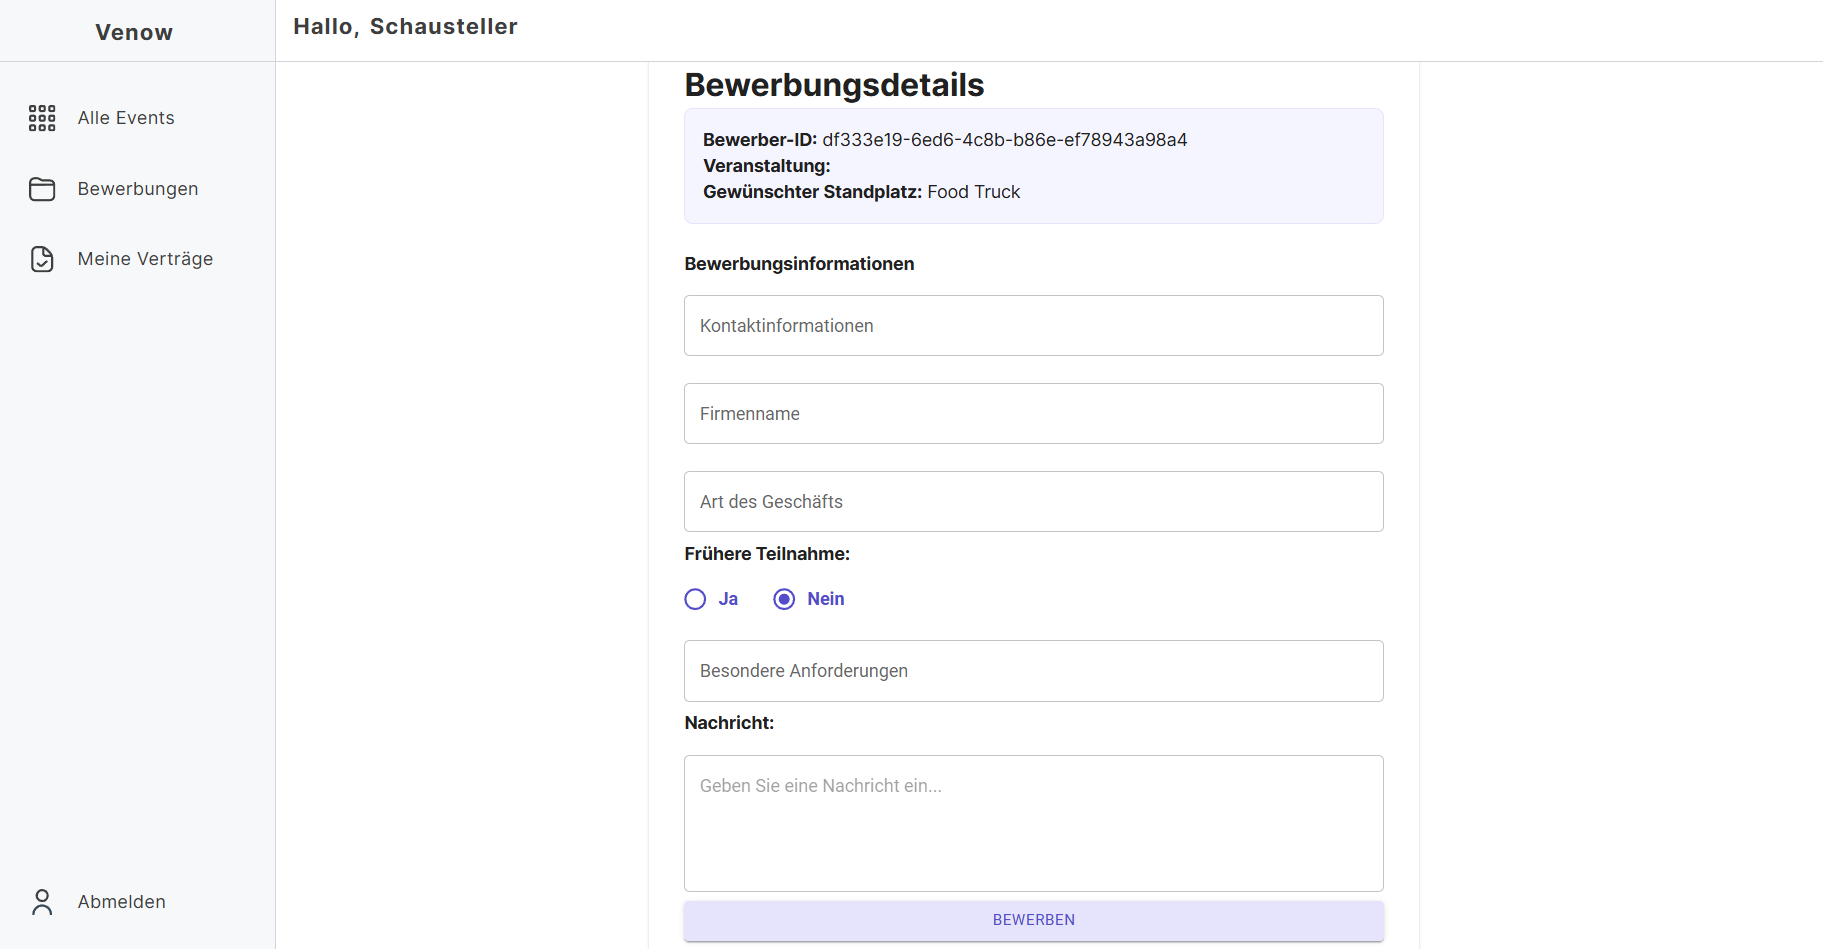
\includegraphics[width=0.8\textwidth]{fig/frontend-exhibitor-apply.png}
	\caption{Bewerbungsformular für Schausteller}
	\label{fig:exhibitor-apply}
\end{figure}

\subsection{Vertragsverwaltung}

Veranstalter können aus einer angenommenen Bewerbung einen Vertrag erstellen. Dabei werden Details wie Preis und Standplatznummer festgelegt. Schausteller erhalten den Vertrag digital und können diesen einsehen. Sie haben die Möglichkeit, den Vertrag zu akzeptieren oder abzulehnen. Sobald beide Parteien den Vertrag annehmen, ist der Bewerbungsprozess abgeschlossen.

\begin{figure}[h]
	\centering
	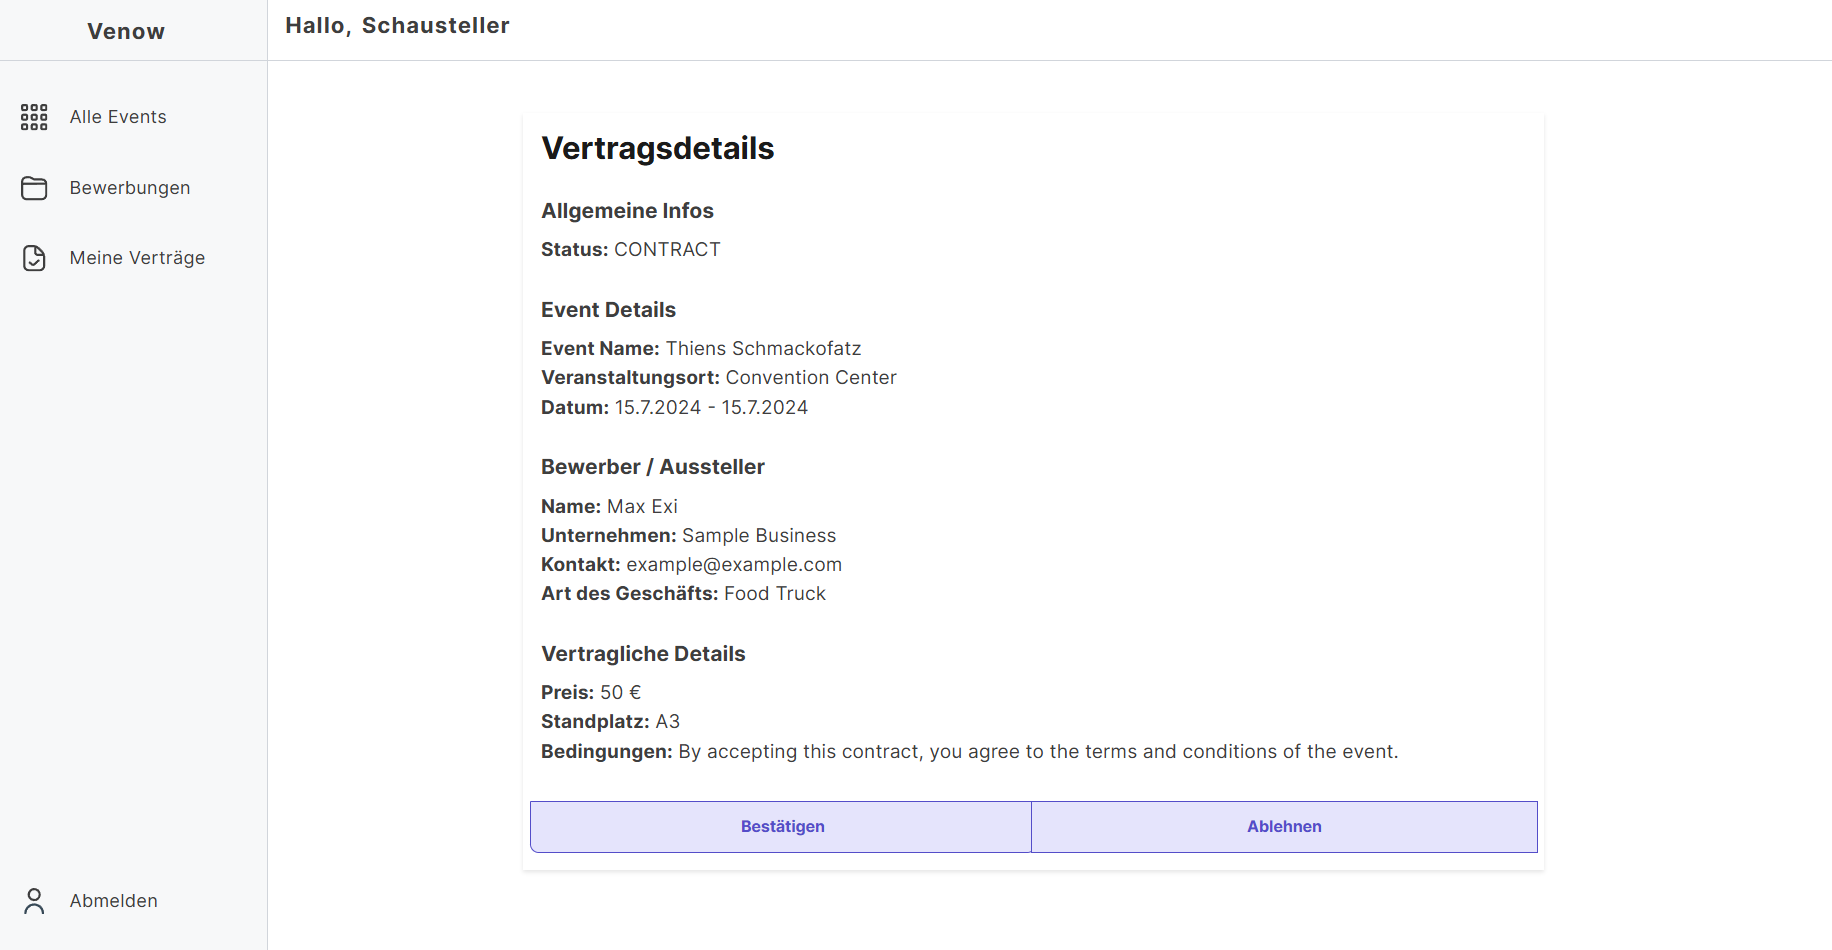
\includegraphics[width=0.8\textwidth]{fig/frontend-exhibitor-contracts-confirm.png}
	\caption{Vertragsdetails für Schausteller}
	\label{fig:exhibitor-contracts}
\end{figure}

\subsection{Veranstaltungs-Management}

Veranstalter können neue Veranstaltungen erstellen und bestehende Veranstaltungen bearbeiten. Alle Veranstaltungen sind für Schausteller sichtbar. Eine integrierte Suchfunktion ermöglicht es, gezielt nach Events zu suchen. Veranstalter können relevante Veranstaltungsdaten wie Datum, Ort und verfügbare Standplätze erfassen. Diese Informationen sind mit anderen Modulen verknüpft. Alle Prozessschritte greifen ineinander, um eine effiziente Verwaltung zu ermöglichen.

\begin{figure}[h]
	\centering
	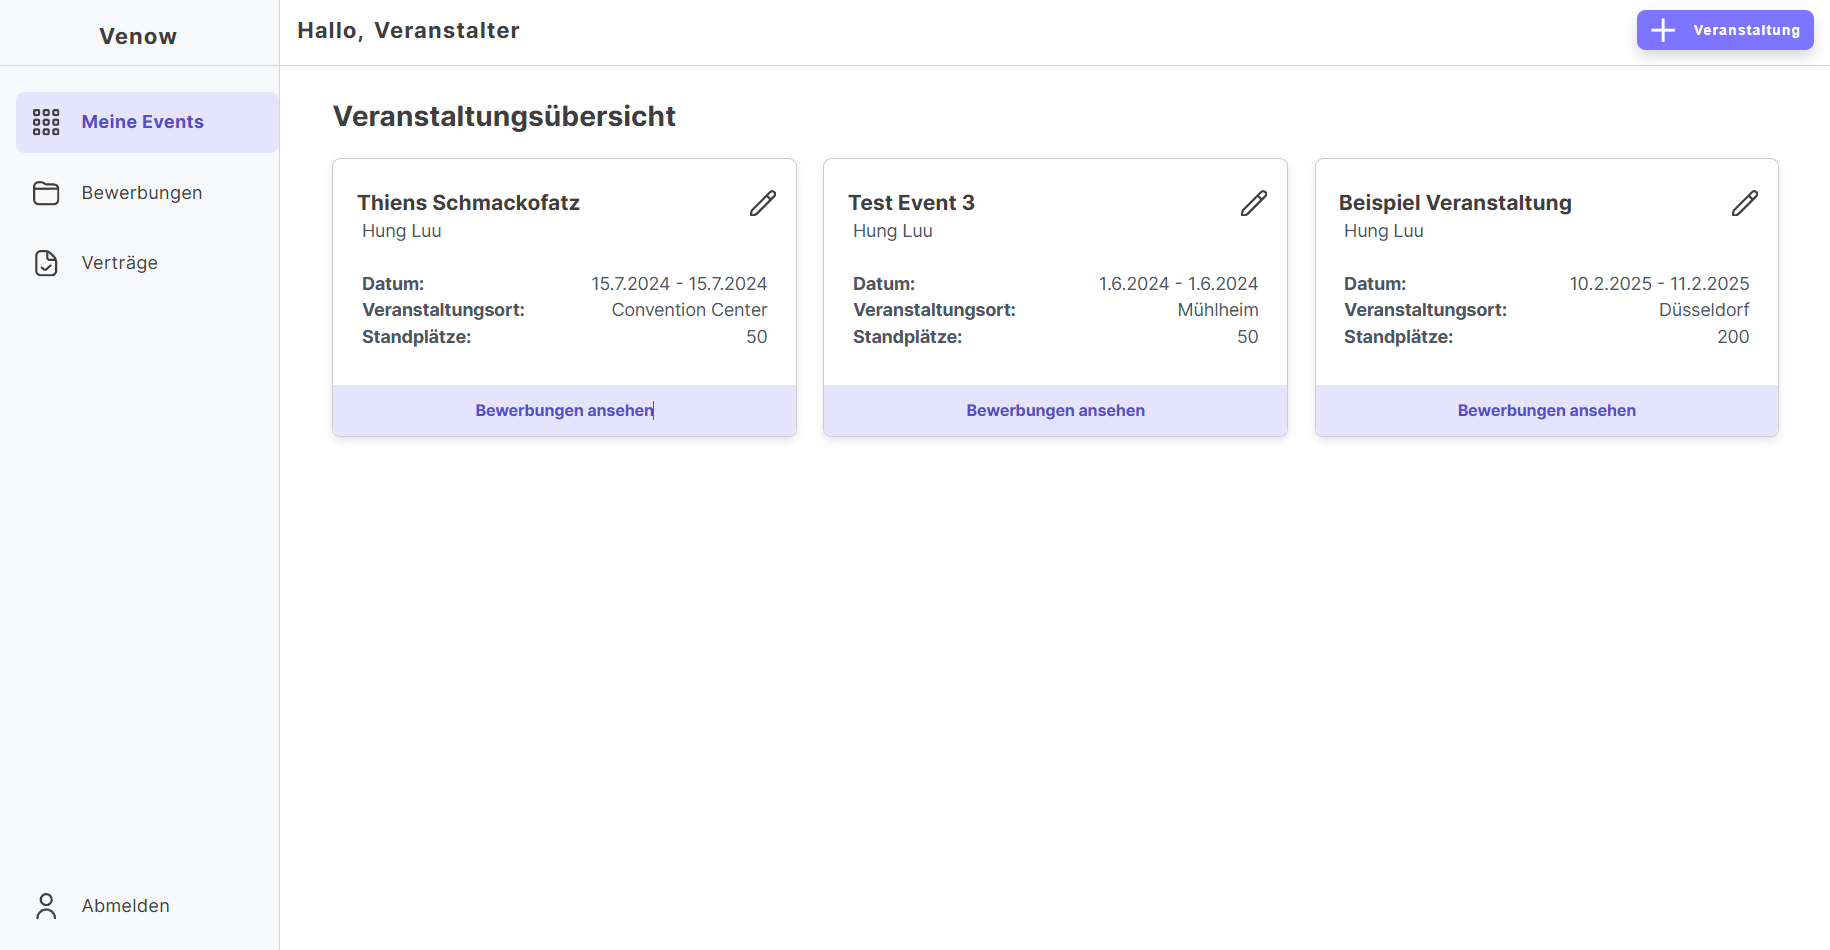
\includegraphics[width=0.8\textwidth]{fig/frontend-organizer-events.png}
	\caption{Übersicht der Events für Veranstalter}
	\label{fig:organizer-events}
\end{figure}

\subsection{Bewerbungen verwalten und Verträge erstellen}

Veranstalter können Bewerbungen prüfen und über eine Annahme oder Ablehnung entscheiden. Wird eine Bewerbung angenommen, kann der Veranstalter direkt einen Vertrag über die Plattform erstellen.

\begin{figure}[h]
	\centering
	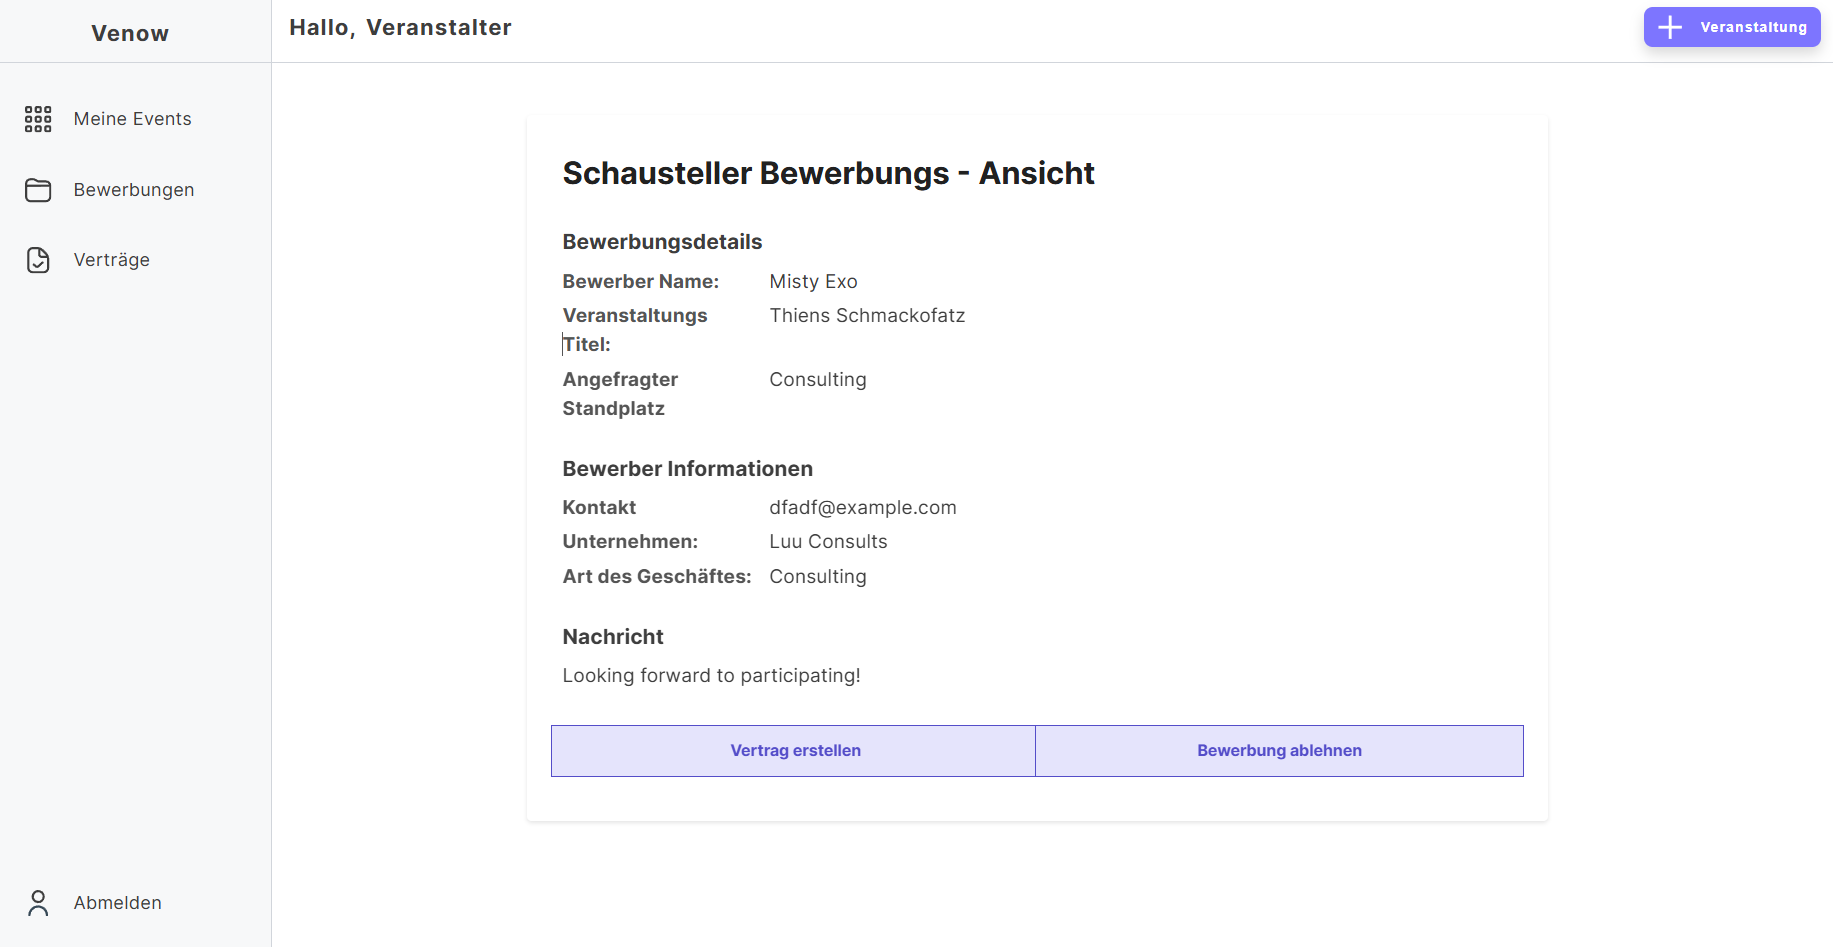
\includegraphics[width=0.8\textwidth]{fig/frontend-organizer-applications-create-contract.png}
	\caption{Ansicht einer Bewerbung mit der Möglichkeit zur Vertragserstellung}
	\label{fig:applications-create-contract}
\end{figure}

\subsection{Erstellung von Events durch Veranstalter}

Veranstalter haben die Möglichkeit, über ein strukturiertes Formular neue Events anzulegen. Hier können sie alle relevanten Informationen wie Datum, Standort und verfügbare Stellplätze erfassen.

\begin{figure}[h]
	\centering
	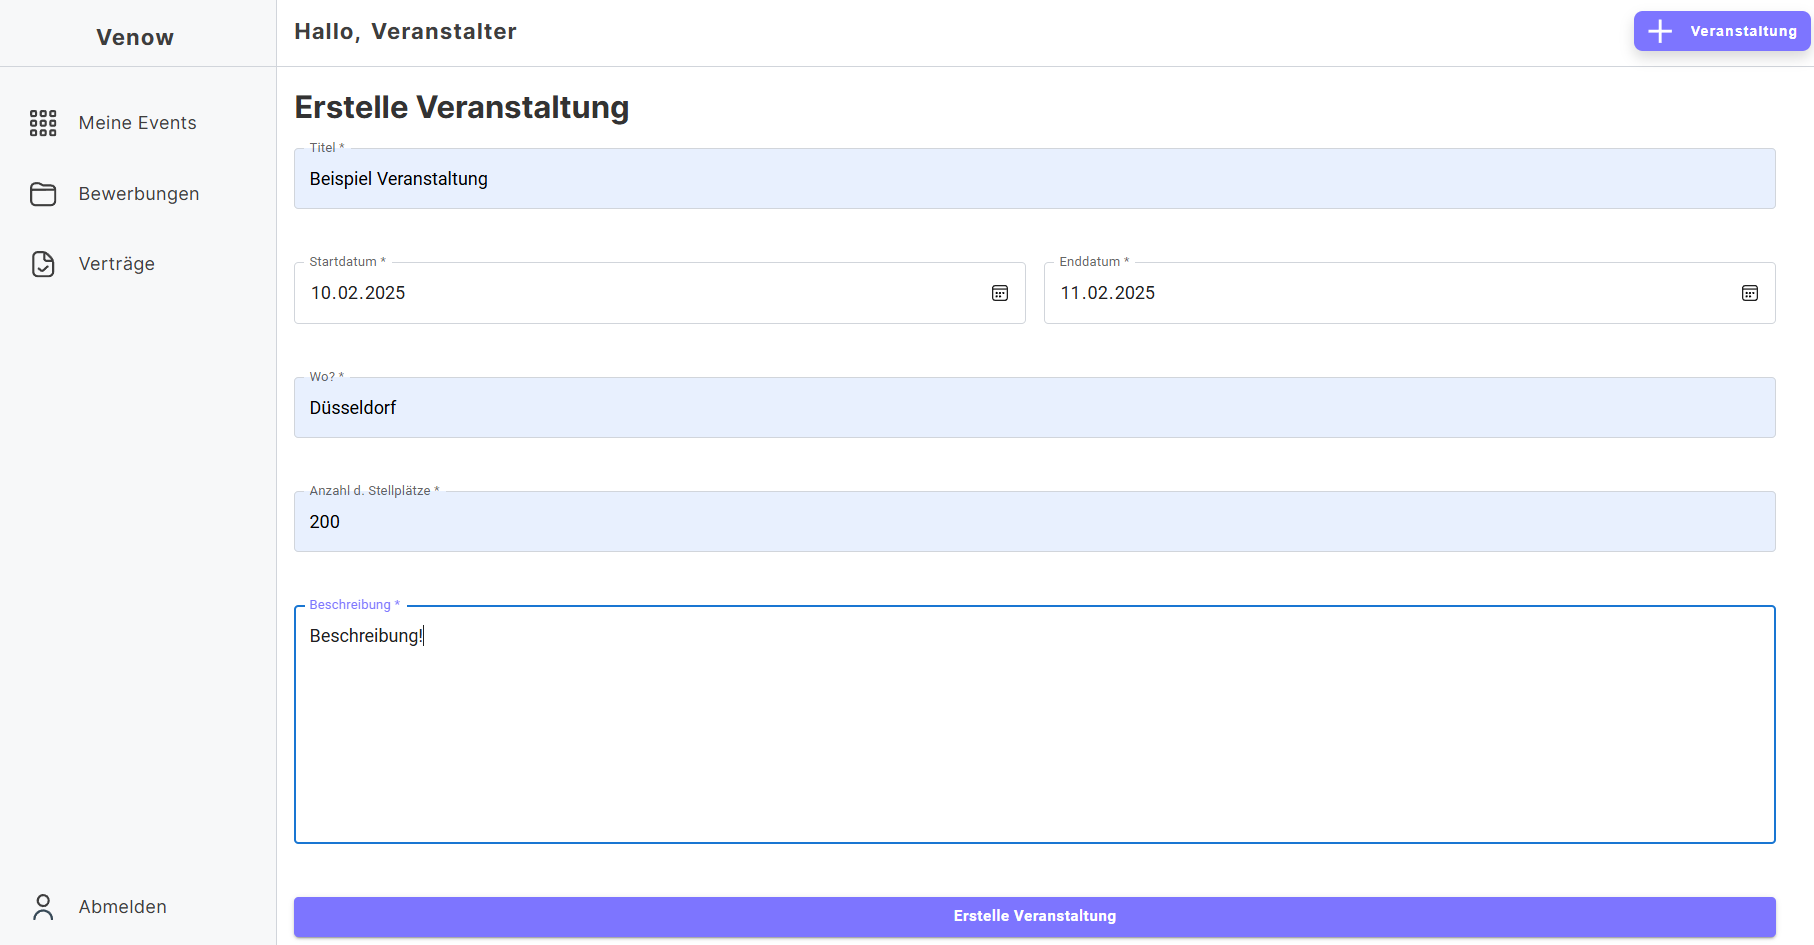
\includegraphics[width=0.8\textwidth]{fig/frontend-organizer-events-create.png}
	\caption{Formular zur Event-Erstellung durch Veranstalter}
	\label{fig:organizer-events-create}
\end{figure}

\subsection{Login-Funktion und grundlegendes Veranstaltungsmanagement}

Die Webanwendung enthält eine Login-Funktion, die den Zugriff auf registrierte Nutzer beschränkt. Dadurch wird sichergestellt, dass nur autorisierte Personen Bewerbungen und Verträge verwalten können. Veranstalter können ihre Veranstaltungen kontinuierlich aktualisieren. Die Plattform stellt sicher, dass alle Prozesse digital und nachvollziehbar bleiben.
Die detaillierte Beschreibung dieser Anwendungsfälle bildet die Grundlage für die spätere Analyse der Teststrategien. Insbesondere wird untersucht, wie sich die Implementierung der verschiedenen Module auf die Effizienz und Effektivität der Tests auswirkt.
